\section{検証方法}
本実験は,層状4分割交差検証を行い,4回の平均をとることで,モデルの汎化性能を評価する.
ただし,一般的な交差検証とは本実験の趣旨や構成が異なるため,以下にその詳細を記す.

\subsection{一般的な層状K分割交差検証}
K分割交差検証とは,用意された学習用とテスト用のデータのうち,学習用のデータをK個にランダムに分割し,そのうちの1つを検証用として用いることをK個のデータそれぞれに対して繰り返し,K回のうち最も精度の良いモデルのパラメータを用いて,まだモデルが見たことがないデータであるテストデータを用いて汎化性能を評価する手法である.\\

層状K分割交差検証とは,クラスごとのサンプル数の比率を保ったまま,K分割交差検証を行う手法である.
これは,データの分布が不均衡な場合に,少数派クラスが学習用データの方に偏ってしまい,評価に使えるサンプルが少なくなることを防ぐためである.


\subsection{本実験における層状K分割交差検証}
本実験における交差検証を\ref{fig:k-fold}に示す. は,学習用とテスト用のデータをK分割し,そのうちの1つをテスト用として用いることをKこのデータそれぞれに対して繰り返し,K回の精度の平均値を評価する.
このようにするのは,本実験で評価する対象が不均衡データであるがために,評価に使う少数派データがごく少数である.その結果,一般的な交差検証ではどのサンプルをテストに用いるかによって精度が大きく変わってしまう可能性が高い.全てのデータを交互にテストデータとして用いることで,モデルの評価がサンプルの質に影響されるのを防ぐ.\\
本実験で扱うデータセットは,全て不均衡なデータのため,層状K分割交差検証を用いた.

\begin{figure}
    \centering
    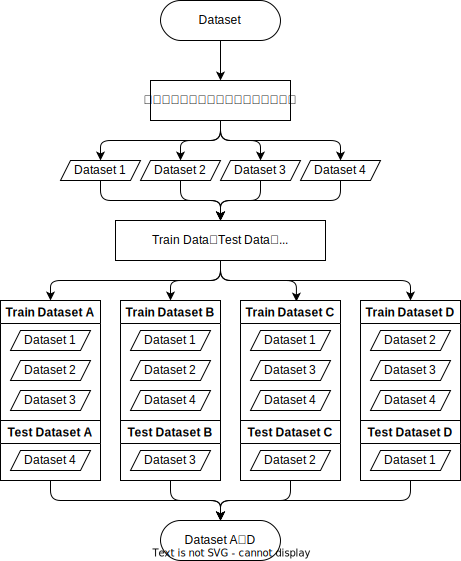
\includegraphics[width=10cm]{figures/stratified-k-fold.png}
    \caption{本実験における層状K分割交差検証}
    \label{fig:k-fold}
\end{figure}

\subsection{ハイパーパラメータチューニング}
ハイパーパラメータチューニングとは,モデルのハイパーパラメータを最適化することで,モデルの汎化性能を向上させる手法である.
本研究では,ハイパーパラメータチューニングを行なったモデルと,行わずにデフォルトのハイパーパラメータで構築したモデルの両方で,精度を測った.
ハイパーパラメータチューニングでは,学習データをさらに3:1に分割し,それぞれを学習と検証に用いる.ただし,計算リソースの都合上,学習データが多いデータセットについては,学習データを30,000件に制限し,残りを検証データとした.
ハイパーパラメータチューニングには,PythonライブラリのOptunaを用いた.
本実験におけるハイパーパラメータチューニングの処理の流れを\ref{fig:hyperparameter-tuning}に示す.


\begin{figure}
    \centering
    \includegraphics[width=15cm]{figures/optuna.png}
        \caption{ハイパーパラメータチューニングの処理の流れ}
        \label{fig:hyperparameter-tuning}
\end{figure}



\subsection{オートエンコーダの構成}
オートエンコーダは,全ての実験において統一して,エポック数10, バッチサイズ32,全ての層の活性化関数にReLU, 最適化関数Adam, 損失関数MSEで学習を行った.\\
ReLUは,ニューラルネットワークにおいて,計算コスト面や,勾配消失問題の解決のために,特に有用な関数として知られており,式\ref{eq:relu}で表される.
\begin{equation}
    \label{eq:relu}
    f(x) = \begin{cases}
        x & (x > 0) \\
        0 & (x \leq 0)
    \end{cases}
\end{equation}

Adamは,勾配降下法の一種である.学習率を動的に変化させることで,学習の収束を早めることができる.\\
MSEは,二乗誤差を表す損失関数である.式\ref{eq:mse}で表される.
\begin{equation}
    \label{eq:mse}
    MSE = \frac{1}{n}\sum_{i=1}^{n}(y_i - \hat{y_i})^2
\end{equation}
ここで,$y_i$は入力値,$\hat{y_i}$は出力値であり,$n$はデータ数である.\\
